\documentclass[12pt,twoside]{article}

\usepackage{template}

\usepackage{Sweave}
\begin{document}
\Sconcordance{concordance:report.tex:report.Rnw:%
1 10 1 1 0 68 1 1 18 19 1 1 8 15 1 1 17 19 1 1 29 14 0 1 2 1 1 1 22 10 %
1 1 25 10 1 1 9 14 1 1 4 20 0 1 2 13 1}


%\begin{titlepage}
\newcommand{\HRule}{\rule{\linewidth}{0.5mm}} 

\center % Center everything on the page

%	TITLE SECTION

\mbox{ }
\vspace{75mm}

%\HRule \\[0.8cm]
{ \Huge \bfseries \color{black}{Analysis of whistler weather data}}\\[0.4cm] 
%\HRule \\[1.5cm]

{\Large
\textsl{Stat 300 Project, Fall 2015}}

\bigskip
{\Large
by Nathan Esau, Ethan Sim, Benjamin Chan}

\vfill

%\vspace{15mm}
%\begin{figure}[!ht]
%\begin{center}
%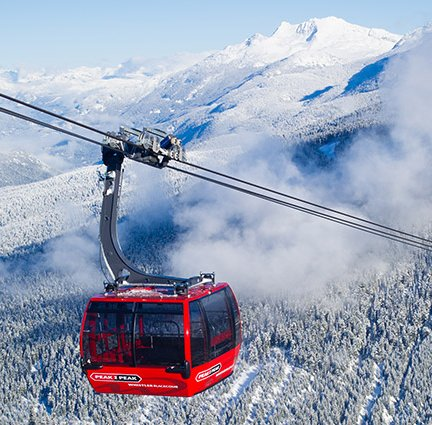
\includegraphics[width=0.9\textwidth]{tp_picture.jpg}
%\end{center}
%\end{figure}

%\vfill
%{\large
%Stat 300 Group Project \\ 
%\medskip
%Fall 2015}

\end{titlepage}

\thispagestyle{firststyle}
\noindent
{\Large \textbf{Analysis of Whistler Weather Data}} 

\medskip\noindent
{\large \textsl{by Benjamin Chan, Ethan Sim and Nathan Esau}}

\section{Summary}

In this study we analyze daily weather data from Whistler, BC obtained from \url{http://climate.weather.gc.ca/}. Data was recorded at an elevation of 657.80 metres, a longitude of 122$^{\circ}$57'17.400'' W and a latitude of 50$^{\circ}$ 07'44.001'' N over the period 2006 -- 2014. The variables analyzed were the amount of snow on the ground, the average temperature during each day and the total precipitation.

\medskip\noindent
Our study was motivated by trying to answer the following questions:

\begin{enumerate}
\item When is the winter season? When does it start, peak and end?
\item How severe is the winter? How much snow is present at different points in the year? 
\item What trends exist in the data? What odd behaviors have shown up over the past 9 years? 
\end{enumerate}

\noindent
To answer our study questions, we used the following techniques:

\begin{enumerate}
\item Regression, to determine whether there was a trend in the snowfall data
\item Time series techniques, such as average smoothing, to compare different winter seasons
\item Correlation, to determine how different variables were related
\end{enumerate}

\noindent We found that while temperature is very consistent year to year, the amount of snowfall has been showing a downward trend. In particular, the 2009--2010 winter in which Vancouver hosted the Olympics was far less severe, both in the amount of snow and the duration of snowfall, than typical winter seasons. This was shown by comparing the 2009--2010 to an average winter at each point in the year, by comparing the length of the winter to other years, and by comparing the peak snowfall and average snowfall to other years.

By averaging the different annual time series, we determined a typical length of a winter season in Whistler. This was done in two ways. First, we classified winter as the period when the snow present on the ground is above a given threshold. Second, we classified winter as the period when temperature stays below a given threshold. This contrasts the typical definition of winter as the period from December 21 to March 21.

These two approaches produced similar results. Under each approach, we found that the 2009--2010 winter was less severe then other winters and that the 2013--2014 winter was shorter than other winters. We also found that the amount of snowfall is correlated with how cold the winter is.

\pagebreak

\section{Introduction}


\end{document}
